\documentclass[12pt,a4paper]{article}
\usepackage{lmodern}
\usepackage{tikz}
\usepackage{pgfplots}
\usepackage{filecontents}
\pgfplotsset{compat=newest}

\usepackage[pdfborder={0 0 0}]{hyperref} % Enveler le cadre rouge des refs

\usepackage[utf8]{inputenc}
\usepackage[T1]{fontenc}
\usepackage[french]{babel}
\usepackage{graphicx}
\usepackage{fancyhdr}
\usepackage{geometry}
\usepackage{titlesec}
\usepackage{amsfonts} % Ensemble mathématique
\usepackage{amsmath} % Environnement mathématique équation
\usetikzlibrary{patterns}
% Configuration de la page
\usepackage{multirow} % Utile pour les tableaux
\usepackage{tabularx}
\usepackage{colortbl}
\usepackage{array}

% Dessin en Latex
\usepackage{tikz}
\usepackage{tikz-3dplot}
\usetikzlibrary{matrix, calc, backgrounds, decorations.pathreplacing}
\usetikzlibrary{3d}

% Couleur : 

\definecolor{myred}{rgb}{1,0,0}

\usepackage{listings}
\geometry{
	top=2cm,
	bottom=2cm,
	left=2cm,
	right=2cm,
	headheight=15pt,
	includeheadfoot
}

% Configuration des en-têtes et des pieds de page
\pagestyle{fancy}
\fancyhf{}
\renewcommand{\headrulewidth}{0.5pt}
\fancyhead[L]{ \textbf{Diffraction des rayons X}}


\fancyfoot[C]{Polytech Clermont-Ferrand -- RX GP4A 2023-2024 \hspace{0.5cm} \textbf{\thepage}}

\fancypagestyle{plain}{
	\fancyhf{}
	\renewcommand{\headrulewidth}{0.4pt}
	\fancyfoot[C]{Polytech Clermont-Ferrand -- RX GP4A 2023-2024 \hspace{0.5cm} \textbf{\thepage}}
}


\renewcommand{\footrule}{\hrulefill} % Dessine la barre horizontale

% Configuration des titres de sections
\titleformat{\section}[hang]{\normalfont\large\bfseries}{\thesection.}{0.5em}{}

\setlength{\parskip}{0.5em}
\title{TP DIFFRACTION DES RAYONS X}
\author{\textup{Vincent MARAIS \\
		Yanis MAURICE}}


% Début du document
\begin{document}
	
% Première page

\begin{titlepage}
	\newcommand{\HRule}{\rule{\linewidth}{0.5mm}}
	\centering 
	\quad\\[1.5cm]


	\makeatletter
	\HRule \\[0.4cm]
	{ \huge \bfseries \@title}\\[0.4cm] 
	\HRule \\[1.5cm]
	\begin{minipage}{0.4\textwidth}
		\begin{flushleft} \large
			\emph{Auteurs:}\\
			\@author 
		\end{flushleft}
	\end{minipage}
	~
	\begin{minipage}{0.4\textwidth}
		\begin{flushright} \large
			\emph{Superviseur:} \\
			\textup{M. Lao }
		\end{flushright}
	\end{minipage}\\[1cm]
	\makeatother	
	
	
\includegraphics[width=0.5\linewidth]{Premier_page/polytech_1}

	
	
	
	\vspace{2cm}
	
		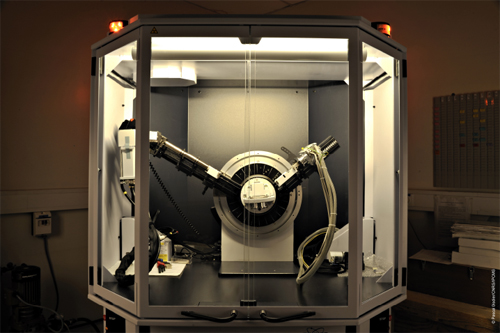
\includegraphics[width=0.7\linewidth]{Premier_page/diffraction-dcmi}


	
	
	
	
	
	
	
	
	\vfill 
	
\end{titlepage}
		


\pagenumbering{roman} % numérotation romaine pour les pages préliminaires
\newpage
\tableofcontents

\newpage
\listoffigures
\listoftables

\newpage
	% Contenu du document
	


\clearpage
\pagenumbering{arabic}

	

	
	
	

\section{Introduction}
	
Durant ce TP, nous avons été introduits à deux méthodes de diffraction des rayons X pour pouvoir étudier la composition d’un matériau.
\begin{flushleft}
	\textbf{Objectifs du TP :}
	
	\textbf{Partie 1 : Réflexion de Bragg :}
	\begin{itemize}
		\item Étude de la réflexion de Bragg sur un monocristal de NaCl avec le rayonnement X caractéristique du molybdène ;
		\item Détermination de la constante de réseau $a_0$ du NaCl ;
		\item Vérification de la loi de la réflexion de Bragg.
	\end{itemize}

\vspace{0.2cm}
	\textbf{Partie 2 : Méthode de Debye-Scherrer :}
	\begin{itemize}
		\item Étude d’un cliché de diffraction  ;
		\item Détermination de la poudre  ;
		\item Calcul de différents paramètres cristallins : distance réticulaire, paramètres de maille, mode de réseau.
	\end{itemize}
\end{flushleft}


\vspace{-0.4cm}
\section{Résultats}

\subsection{Réflexion de Bragg}










\subsubsection{Calcul des longueurs d'ondes des raies $K_{\alpha}$ et $K_{\beta}$ émis par le molybdène}


Tout d'abord, en utilisant le tableau \ref{tab: Tableau des nergies de niveaux lectroniques du Molybdne et du Zirconium}, nous pouvons déduire l'énergie du photon émis par la transition électronique $\Delta E(eV)$. 

\begin{table}[h!]
	\centering
	\begin{tabular}{|l|c|c|c|c|}
		\hline
		\textbf{Énergie des niveaux électroniques (keV)} & K     & $L_{\mathrm{III}}$ &$L_{\mathrm{II}}$ & $M_{\mathrm{III}}$ \\ \hline
		Molybdène      (Mo)                                  & 20.03 & 2.56 & 2.66 & 0.42 \\ \hline
		Zirconium      (Zn)                                  & 18.02 &      &      &      \\ \hline
	\end{tabular}
	\caption{Énergies des niveaux électroniques du molybdène et du zirconium}
	\label{tab: Tableau des nergies de niveaux lectroniques du Molybdne et du Zirconium}
\end{table}


Exemple pour la transition électronique $L_{\mathrm{III}} \to K$ pour le molybdène, on a : 
\vspace{0.2cm}
\begin{equation*}	
	\begin{split}
		\Delta E  & = E(K) - E(L_{\mathrm{III}})  \\
		& = 20.06 - 2.56  \\
		& = 17.47keV
	\end{split}	
\end{equation*}

Ensuite, en appliquant l'équation \ref{eq: Energie_longueur_donde}, on obtient la longueur d'onde du photon émit lors d'une transition électronique.

\begin{equation}\label{eq: Energie_longueur_donde}
	\Delta E(eV) = \frac{1.24}{\lambda (\mu m)}
\end{equation}

\newpage
Et enfin, on réalise le tableau \ref{tab: Transition nergitique en les diffrentes couche du molybdne et les diffrentes longueurs donde misse par les transitions}. 
\begin{table}[h!]
	\centering
	\begin{tabular}{|c|c|c|}
		\hline
		\multicolumn{1}{|l|}{\textbf{Transition}} & \multicolumn{1}{l|}{\textbf{Energie (keV)}} & \multicolumn{1}{l|}{\textbf{Longueur d'onde}} \\ \hline
		$L_{\mathrm{III}} \to K \ (K_{\alpha_1}) $                    & 17.47                                       & 0.709 \AA                                       \\ \hline
		$L_{\mathrm{II}} \to K \ (K_{\alpha_2}) $                      & 17.37                                       & 0.713 \AA                                       \\ \hline
		$M_{\mathrm{III}} \to K \ (K_{\beta}) $                         & 19.61                                       & 0.632 \AA                                       \\ \hline
	\end{tabular}
	\caption{\centering Longueurs d'ondes des rayons X émis par le molybdène lors des transitions électroniques $K_{\alpha}$ et $K_{\beta}$}
	\label{tab: Transition nergitique en les diffrentes couche du molybdne et les diffrentes longueurs donde misse par les transitions}
\end{table}





\subsubsection{Mesure de l’intensité ($I$) en fonction de l’angle ($\theta$)}
Dans cette partie, nous allons analyser le plan (200) d'un monocristal de NaCl à l'aide d'un système de diffraction des rayons X (figure \ref{fig:machine-diffraction-rx})

\begin{figure}[h!]
	\centering
	\includegraphics[width=0.7\linewidth]{"Réflexion de Bragg/Machine diffraction RX"}
	\caption{\centering Photo du système de diffraction des rayons X avec (1) : collimateur, (2) : filtre de Zn, (3) : monocristal de NaCl, (4): Compteur Geiger Muller, (5) : angle $\theta$, (6) : rayon X, (7) : plan (200) du monocristal de NaCl }
	\label{fig:machine-diffraction-rx}
\end{figure}



Pour analyser le plan (200) du monocristal de NaCl, le système de diffraction des rayons X déplace le système \{tube compteur + monocristal\} d'un angle $\theta$. Pour notre analyse, nous aurons $\theta$ compris dans l'intervalle $[4^\circ, 24^\circ]$ avec un pas de $\Delta \theta = 0.1^\circ$. De plus, dans un premier temps, nous réaliserons la mesure sans le filtre au Zn, puis nous effectuerons une seconde mesure avec le filtre et commenterons les effets de ce filtre sur la réponse.












\newpage

L'objectif de cette partie est déterminer le paramètre de maille $a_0$ de la maille de NaCl représentée sur le figure \ref{fig:cristalnacl}
\begin{figure}[h!]
	\centering
	
\tdplotsetmaincoords{75}{110} % Définir les angles de vue
\begin{tikzpicture}[scale=2, tdplot_main_coords,axis/.style={->},thick]  
	
	\foreach \x in {0,1,2}
	\foreach \y in {0,1,2}
	\foreach \z in {0,1,2}
	{
		\draw[thick,opacity=1] (\x,0,\z) -- (\x,2,\z);
		\draw[thick,opacity=1] (0,\y,\z) -- (2,\y,\z);
		\draw[thick,opacity=1] (\x,\y,0) -- (\x,\y,2);
	}
	% --- labels for vertices
	\foreach \x in {0,1,2}
	\foreach \y in {0,1,2}
	\foreach \z in {0,1,2}
	{\draw[fill=gray!50] (\x,\y,\z) circle (0.3em);}    
	
	\foreach \x/\y in {1/0,2/1,1/2,0/1}
	\foreach \z in {0,2}
	{\draw[fill=orange] (\x,\y,\z) circle (0.4em);}
	
	\foreach \x/\y in {2/0,2/2,0/2,0/0}
	\foreach \z in {1}
	{\draw[fill=orange] (\x,\y,\z) circle (0.4em);}
	
	\foreach \x/\y in {1/0,2/1,1/2,0/1}
	\foreach \z in {1}
	{\draw[fill=gray!50] (\x,\y,\z) circle (0.3em);}
	
	\foreach \x/\y in {1/1}
	\foreach \z in {0,2}
	{\draw[fill=gray!50] (\x,\y,\z) circle (0.3em);}
	
	\foreach \x/\y in {1/1}
	\foreach \z in {1}
	{\draw[fill=orange] (\x,\y,\z) circle (0.4em) ;}
	
	
	\draw[thick,->, red] (2,0,0) -- (0,	0,0) node[pos=0.65,anchor=west]{\(\vec{c}\)};
	\draw[thick,->, red] (2,0,0) -- (2,2,0) node[pos=0.7, anchor=north]{\(\vec{b}\)};
	\draw[thick,->, red] (2,0,0) -- (2,0,2) node[pos=0.9, anchor=west]{\(\vec{a}\)};
	
	\draw (2, -1, 1.5) node[circle,fill=orange,scale=0.5] {} node[anchor=south west] {Cl$^-$};  
	
	\draw (2, -1, 2) node[circle,fill=gray!50,scale=0.5] {} node[anchor=south west] {Na$^+$};  
	
	\filldraw[fill=green!50!black, opacity=0.5] (2,2,1) -- (0,2,1) -- (0,0,1) -- (2,0,1) -- cycle;
	
	\draw (2.5, 3, 2) node[anchor=south west, green!50!black] {(200)};  
	
	\draw[thick,-, blue] (2,2,0) -- (2,	2,1) node[pos=0.77,anchor=west]{\(d_{200}\)};
	
	\draw[thick,-, blue] (0,2,0) -- (0,	2,2) node[pos=0.3,anchor=west]{\(a_0\)};
\end{tikzpicture}


% Dans cet exemple, j'ai utilisé pos=1.1, ce qui place le "node" juste après la fin du vecteur (à 110% du chemin, pour ainsi dire). L'anchor=west signifie que le côté ouest (gauche) du "node" est aligné avec ce point.  %
	\caption{\centering Maille de NaCl de paramètre de maille $a_0$, $\left(\vec{a}, \vec{b}, \vec{c}\right)$ : base directe du réseau réel de la maille de NaCl.}
	\label{fig:cristalnacl}
\end{figure}







Après avoir lancé l'expérience grâce au système présenté figure \ref{fig:machine-diffraction-rx}, nous obtenons la figure \ref{fig:spectre-de-diffraction-de-nacl}





\begin{figure}[h!]
	\centering
	\includegraphics[width=1\linewidth]{"Réflexion de Bragg/Spectre de diffraction de NaCl"}
	\caption{\centering Spectre en intensité du monocristal en fonction de l'angle $\beta$ équivalent à l'angle $\theta$ de la figure \ref{fig:machine-diffraction-rx}, \textbf{courbe noir} : Spectre sans le filtre Zn, {\color{red}\textbf{courbe rouge}} : Spectre avec le filtre Zn, $ {\color{blue} \theta_1} = 6.4^\circ$ : angle de diffraction de la 1ère raie et $ {\color{blue} \theta_2}=7.2^\circ$ : angle de diffraction de la 2nd raie  }
	\label{fig:spectre-de-diffraction-de-nacl}
\end{figure}



	
\subsubsection{Interprétation de la mesure de l’intensité ($I$) en fonction de l’angle ($\theta$)}
Dans tout la suite nous parlons de spectre en intensité avec l'intensité du rayon X incident est proportionnel aux nombre de coup par second comptabilisé par le compteur Geiger Muller présent sur la figure \ref{fig:machine-diffraction-rx}.
	
\begin{flushleft}
	\textbf{Type de transition électronique pour la première raie}	
\end{flushleft}

Dans un premier temps, nous pouvons affirmer que nous obtenons la diffraction d'angle $\theta_1$ d'un photon dû à une transition $K_{\beta}$, car la longueur d'onde émise par ce photon lors de cette transition est la plus courte par rapport à celle émis lors d'une transition $K_{\alpha_1}$ ou $K_{\alpha_2}$ d'après le tableau \ref{tab: Transition nergitique en les diffrentes couche du molybdne et les diffrentes longueurs donde misse par les transitions}.

Conformément à la loi de Bragg (équation \ref{eq:Loi_de_Bragg}) il y a nécessité d'un angle faible pour la raie $K_{\beta}$ justifie donc que la première raie observée est bien une $K_{\beta}$.

\begin{flushleft}
	\textbf{Type de transition électronique pour la seconde raie}	
\end{flushleft}

\textbf{Raisonnement par l'absurde : } supposons que la seconde raie visible soit une $K_{\beta}$. \textbf{(H)} \

\vspace{0.2cm}

Cela signifie donc que la seconde raie est d'ordre de diffraction $n=2$ correspondant avec un angle de diffraction $\theta_2$.
Ainsi, en appliquant la loi de Bragg (\ref{eq:Loi_de_Bragg}) au plan (200) pour un photon émis lors d'une transition $K_{\beta}$ de longueur d'onde $\lambda_{K_{\beta}} = 0.632 \ \AA$ (tableau \ref{tab: Transition nergitique en les diffrentes couche du molybdne et les diffrentes longueurs donde misse par les transitions}) et diffracté sous un angle $\theta_{2}$, nous avons :
\begin{equation} \label{eq: photon K_beta + Bragg}
	\frac{\lambda_{K_{\beta}}}{2d_{200}}=\frac{\sin(\theta_{2})}{2}
\end{equation}

Cependant, nous avons démontré que la première raie était dû à photon émis par une transition de type $K_{\beta}$, donc pour cette raie on a $n=1$ et un angle de diffraction $\theta_{1}$, et donc d'après la loi de Bragg (\ref{eq:Loi_de_Bragg}) :

\begin{equation} \label{eq: constant Bragg}
	\frac{\lambda_{K_{\beta}}}{2d_{200}}=\sin(\theta_{1}) = cte
\end{equation}

Par conséquent, selon (\ref{eq: constant Bragg}) et (\ref{eq: photon K_beta + Bragg}), nous obtenons :

\begin{equation}
	\frac{\sin(\theta_{2})}{2} = \sin(\theta_{1})
\end{equation}

Cependant, après calcul à l'aide de la figure  \ref{fig:spectre-de-diffraction-de-nacl} :
\begin{equation}
	\frac{\sin(\theta_{2})}{2} = 0.063 \ \text{et } \sin(\theta_{1}) = 0.111
\end{equation}



Donc :
\begin{equation} \label{eq:Inegalite_theta}
	\frac{\sin(\theta_{2})}{2} < \sin(\theta_{1})
\end{equation}

Ainsi, $(H)$ n'est pas vérifié, ce qui signifie nécessairement que nous avons une raie $K_{\alpha}$.

\newpage
En appliquant périodiquement ce raisonnement nous obtenons le tableau \ref{tab:Pic_de_diffraction_et_d'interférence_du_cristal_NaCl_sur_le_plan_200}.


\begin{table}[h!]
	\centering
	\begin{tabular}{|c|c|c|c|c|}
		\hline
		$\theta$ (°) & $\sin(\theta)$ &$K_{\alpha}$ ? ou $K_{\beta}$ ? & n & $n \times \lambda $ (pm) \\ \hline
		6.4       & 0.111      & $K_{\beta}$                     & 1 & 63.2 \\ \hline
		7.2       & 0.125      &$K_{\alpha}$                    & 1 & 70.9 \\ \hline
		12.9      & 0.223      & $K_{\beta}$                     & 2  & 126.4\\ \hline
		14.5      & 0.250      &$K_{\alpha}$                    & 2  & 141.8\\ \hline
		19.6      & 0.335      & $K_{\beta}$                     & 3  & 189.6\\ \hline
		22.1      & 0.376      &$K_{\alpha}$                    & 3  & 212.7 \\ \hline
	\end{tabular}	
	\caption{Pics de diffractions et d'interférences du cristal NaCl sur le plan (200)}
	\label{tab:Pic_de_diffraction_et_d'interférence_du_cristal_NaCl_sur_le_plan_200}
\end{table}




Du tableau \ref{tab:Pic_de_diffraction_et_d'interférence_du_cristal_NaCl_sur_le_plan_200}, on trace la figure \ref{fig:courbetendance} et l'aide du programme Python (cf figure \ref{fig:photocode})


\begin{figure}[h!]
	\centering
	\includegraphics[width=1.1\linewidth]{"Réflexion de Bragg/Courbe_tendance"}
	\caption{Courbe de tendance de $n \times \lambda $ (pm) et fonction de 	$\sin(\theta)$ }
	\label{fig:courbetendance}
\end{figure}


De cette courbe nous pouvons en déduire le paramètre de maille $a_0$ du monocristal car d'après la figure \ref{fig:cristalnacl} on a :
	
	\begin{equation}\label{eq: paramètre de maille et d_200}
		a_0=2d_{200}
	\end{equation}

	
De plus, si on applique la loi de Bragg (équation \ref{eq:Loi_de_Bragg}) au plan $(200)$ du monocristal de NaCl, on obtient : 

\begin{equation} \label{eq:Loi_de_Bragg_NaCl_200}
	\sin (\theta ) = \frac{n \lambda }{2 d_{200}}
\end{equation}
	
	
Donc, d'après (\ref{eq: paramètre de maille et d_200}) l'équation (\ref{eq:Loi_de_Bragg_NaCl_200}) devient :
	
	\begin{equation}\label{eq: Bragg et paramètre de maille}
		n \times \lambda = a_0sin(\theta)
	\end{equation}
	
	
	Par conséquent, d'après l'équation (\ref{eq: Bragg et paramètre de maille}), $a_0$ est le coefficient directeur de la courbe  de tendance tracer sur la figure \ref{fig:courbetendance}, on en déduit donc :
	
	\begin{equation} \label{eq: paramètre de maille NaCl avec système RX}
		\boxed{a_0 = 564.6 \ pm}
	\end{equation}
	




%%% Interprétation 
 \begin{flushleft}
	\textbf{Vérification de la valeur de $a_0$:}
\end{flushleft}



En représentant le plan (200) du monocristal de NaCl vu de dessus, nous obtenons la figure \ref{fig:Plan (200) du monocristal de NaCl vu de dessus} en supposant que le cristal respecte ses deux règles de stabilité :

\begin{itemize}
	\item Il y a un contact (ou tangence) entre les ions $Na^+$ et $Cl^-$ les plus proches voisins;
	\item Il n'existe aucun contact entre anions-anions ou cations-cations.
\end{itemize}
	



	

\begin{figure}[h!]
	\centering
\begin{tikzpicture}
	
	
	
	% Blue Circles
	\foreach \pos in {(0,0) , (-1.8,-1.8), (1.8,1.8), (1.8,-1.8), (-1.8,1.8)} {
		\draw[fill=orange] \pos circle (1.25);
	}
	
	\foreach \pos in {(0,1.8), (0,-1.8), (-1.8,0), (1.8,0) } {
		\draw[fill=gray!50] \pos circle (0.55);
	}
	% Lines
	
	% Légende
	\draw (4, 0) node[circle,fill=orange,scale=0.5] {} node[anchor=south west] {Cl$^-$};  
	
	\draw (4, -1) node[circle,fill=gray!50,scale=0.5] {} node[anchor=south west] {Na$^+$};  
	
	\draw[thick,->, black] (0,0) -- (0.89,0.89) node[pos=0.3,anchor=west]{\(r_{Cl^-}\)};
	
	\draw[thick,->, black] (0,1.8) -- (0.15,2.33) node[pos=0.3,anchor=north]{\(r_{Na^+}\)};
	% Label
	
	\draw[very thick,<->, blue] (-1.8,-1.8) -- (-1.8,1.8) node[pos=0.2,anchor=west]{\(a_0\)};
\end{tikzpicture}
	\caption{\centering Plan (200) du monocristal de NaCl vu de dessus, $r_{Na^+}$ : rayon du cation $Na^+$, $r_{Cl^-}$ : rayon de l'anion $Cl^-$}
	\label{fig:Plan (200) du monocristal de NaCl vu de dessus}
\end{figure}

	
	D'après la figure \ref{fig:Plan (200) du monocristal de NaCl vu de dessus}, on en déduit que :
	
	\begin{equation}
		a_0 = 2r_{Na^+}+2r_{Cl^-}
	\end{equation}

avec 
\begin{itemize}
	\item $r_{Na^+}= 98 \ pm$
	\item $r_{Cl^-}= 181 \ pm $	
\end{itemize}


\vspace{0.2cm}

\begin{flushleft}
	\textbf{Application numérique :}
\end{flushleft}

	
	\begin{equation}
		a_0 = 558 \ pm
	\end{equation}
	
On a un écart de $ \pm \ 6.6\  pm$,  soit une de erreur de $1.1 \ \%$
\begin{flushleft}
	\textbf{Interprétation :}
\end{flushleft}


D'après la figure \ref{fig:courbetendance} nous obtenons une courbe de tendance de la forme :

\begin{equation}
	y=a x + b
\end{equation}
où :
\begin{itemize}
	\item $a =564.6 \ pm$ 
	\item $b = 0.4722 \ pm$
\end{itemize}
\vspace{0.2cm}
Ainsi, cela signifie que lorsque nous avons un rayon X qui arrive de manière colinéaire au plan (200) avec un angle $\theta = 0^\circ$, nous obtenons $n \times \lambda = 0.4722 \ pm$. Il en résulte qu'il existe un rayon X diffracté par le plan (200), ce qui semble incohérent. Cependant, il est possible d'admettre une certaine incertitude sur l'angle $\theta$, ce qui expliquerait pourquoi notre valeur de $b$ n'est pas nulle.



On pose :

\begin{equation}
	R = \frac{\sin(\theta_{K_{\alpha}})}{\sin(\theta_{K_{\beta}})}
\end{equation}


 \begin{flushleft}
	\textbf{Calcul du R (théorique) : $R_{th}$}
\end{flushleft}


Pour le photon émis par une transition électronique $(K_{\alpha})$ de longueur d'onde $\lambda_{K_{\alpha}}$diffracté sur le plan (200) d'un angle $\theta_{K_{\alpha}}$, on obtient la loi de Bragg (\ref{eq:Loi_de_Bragg}) suivante :

\begin{equation}\label{eq: Bragg_photon_K_alpha}
	2 d_{200}\sin(\theta_{K_{\alpha}}) = n\lambda_{K_{\alpha}}
\end{equation}

Pour le photon émis par une transition électronique $(K_{\beta})$ de longueur d'onde $\lambda_{K_{\beta}}$ diffracté sur le plan (200) d'un angle $\theta_{K_{\beta}}$, on obtient la loi de Bragg (\ref{eq:Loi_de_Bragg}) suivante :

\begin{equation}\label{eq: Bragg_photon_K_beta}
	2 d_{200}\sin(\theta_{K_{\beta}}) = n\lambda_{K_{\beta}}
\end{equation}

Donc d'après (\ref{eq: Bragg_photon_K_alpha}) et (\ref{eq: Bragg_photon_K_beta}) on a :
\begin{equation}\label{eq:R_{th}}
	R_{th} = \frac{\lambda_{K_{\alpha}}}{\lambda_{K_{\beta}}} 
\end{equation}


 \begin{flushleft}
	\textbf{Application numérique :}
\end{flushleft}


D'après le tableau \ref{tab: Transition nergitique en les diffrentes couche du molybdne et les diffrentes longueurs donde misse par les transitions} on a :

\begin{equation}\label{eq:A.N lambda}
	\lambda_{K_{\alpha}} = \frac{0.713 + 0.709}{2} = 0.711 \ \AA, \ \lambda_{K_{\beta}} =0.632 \ \AA
\end{equation}

Donc d'après (\ref{eq:R_{th}}) et (\ref{eq:A.N lambda}) on a :  
\begin{equation}\label{eq:R_{th}_A.N}
	R_{th} = 1.125
\end{equation}

\newpage
Ensuite, on calcule la valeur de R mesurée par l'expérience pour chaque ordre de diffraction n en utilisant le tableau \ref{tab:Pic_de_diffraction_et_d'interférence_du_cristal_NaCl_sur_le_plan_200}, puis on les compare à la valeur de $R_{th}$ dans le tableau \ref{tab:R en fonction de n}.





	
	
	
	



\begin{table}[h!]
	\centering
	\begin{tabular}{|c|c|c|}
		\hline
		$R_{th}$& $R$ (mesurée) & $n$ \\ \hline
		1.125 &1.126 & 1 \\ \hline
		1.125 &1.121& 2 \\ \hline
		1.125 & 1.122& 3 \\ \hline
	\end{tabular}
	\caption{R en fonction de n}
	\label{tab:R en fonction de n}
\end{table}




Nous remarquons que la valeur de $R$ (mesurée) $= R_{th}$ au chiffre des millièmes près, ce qui valide la théorie.

 \begin{flushleft}
	\textbf{Intérêt du filtre de Zn}
\end{flushleft}







 
Ensuite, l'intérêt du filtre de Zn consiste à supprimer les raies présentant la plus forte énergie. Lorsqu'un rayonnement X dû à une transition $K_{\beta}$ arrive au filtre de Zn, il possède suffisamment d'énergie pour ioniser l'atome de Zn (effet photoélectrique), entraînant ainsi sa disparition comme le synthétise la figure \ref{fig: Effet photoélectrique de le métal de Zn}. C'est pourquoi, comme on peut le voir sur la courbe rouge de la figure \ref{fig:spectre-de-diffraction-de-nacl}, les pics de $K_{\beta}$ sont fortement atténués, favorisant ainsi le pic de $K_{\alpha}$. 

\begin{figure}[h!]
	\centering
	\begin{tikzpicture}[photon/.style={-stealth,decorate,decoration={snake,post length=1mm}}]
	
	% Dessiner le métal
	\fill[gray!20] (0,0) rectangle ++(6,-2.2);
	\draw[thick] (0,0) -- ++(6,0);
	\node[anchor=north] at (3,0) {Cristal de Zn};
	
	% Dessiner les électrons dans le métal
	\foreach \x/\y in {0.7/-0.5,2/-1.25,4/-1.75/-0.5}{
		\draw (\x,\y) node[circle,fill,inner sep=2pt, color=red,label={east:${\color{red}e^-}$}] {}; 
	}
	
	% Dessiner le photon incident
	\draw[photon,green] (-1,1) -- node[above=4mm,font=\footnotesize] {RX $(K_{\beta})$} ((4,-1.75);
	
	% Dessiner l'électron éjecté
	\draw[-stealth,blue,thick] (4,-1.75) -- node[above=-1mm,font=\footnotesize, sloped] {Électron éjecté} ++(3,2);
	
	
	\draw[<->, thick] (7,0) -- node[midway, right,font=\footnotesize] {Bande de conduction} (7,-1);
	
	\draw[dashed] (6,0) -- (7.5,0);
	
	\draw[dashed] (7,-1) -- (7,-1.5);
	
	\draw[<->, thick] (7,-1.5) -- node[midway, right,font=\footnotesize] {Bande K} (7,-2.2);
	
	\draw[->, thick] (-1,0) -- node[midway, left,font=\footnotesize] {$E(keV)$} (-1,-2.2);
	
	\foreach \y/\x  in {-1/$E_{K_{\alpha}}$, -1.5/$E_{K_{Zn}}$, -2/$E_{K_{\beta}}$} 
	{
		\draw [dashed] (-1,\y) -- (0,\y) node[right] {\x};
		\draw[dashed] (1,\y) -- (7,\y);
	}
	

	
\end{tikzpicture}



	\caption{\centering Effet photoélectrique dans le filtre de Zn , $E_{K_{\alpha}}$ : énergie d'une transition $K_{\alpha}$, $E_{K_{\beta}}$ : énergie d'une transition $K_{\beta}$, $E_{K_{Zn}}$ : niveau d'énergie de la bande K du cristal de Zn avec l'ensemble des énergies sont répertoriés dans les tableaux \ref{tab: Tableau des nergies de niveaux lectroniques du Molybdne et du Zirconium} et \ref{tab: Transition nergitique en les diffrentes couche du molybdne et les diffrentes longueurs donde misse par les transitions}}
	\label{fig: Effet photoélectrique de le métal de Zn}
\end{figure}


De plus, dans le cas d'une analyse plus complexe de plusieurs plans du cristal, cela nous permet de réduire la quantité d'informations reçues par le logiciel, ce qui facilite l'interprétation de la courbe obtenue. Sans le filtre, l'information utile serait répétée deux fois.








\newpage










\subsection{Méthode de Debye-Scherrer ou méthode des poudres}
\vspace{0.2cm}

\subsubsection{Principe de la méthode de Debye-Scherrer}

La méthode de Debye-Scherrer (fig \ref{fig:methodededebyescherrer}) est employée pour déterminer la structure cristalline d'un matériau. Elle implique l'orientation d'un faisceau de rayons X monochromatiques vers un échantillon cristallin, induisant ainsi la diffraction des rayons X par les plans du réseau cristallin. En mesurant les angles de diffraction sur le film, il devient possible de calculer les distances interatomiques et de révéler la structure cristalline de l'échantillon. Enfin, une analyse de l'épaisseur des tâches sur le film nous permet d'établir une corrélation entre le diamètre des anneaux observés et la distance intermoléculaire du plan diffractant de différentes espèces chimiques.





\begin{figure}[h!]
	\centering
	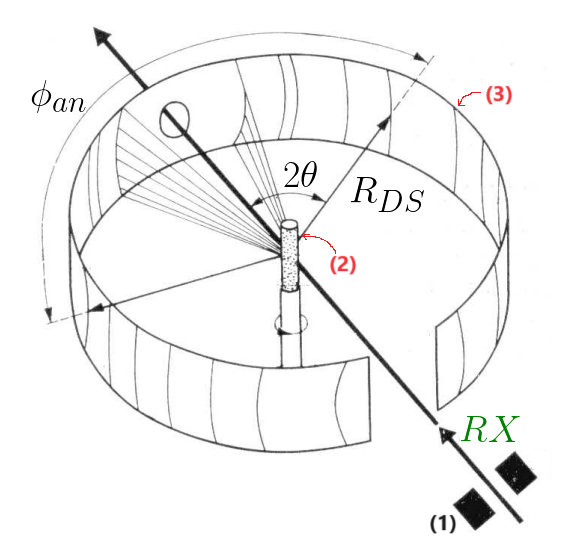
\includegraphics[width=0.6\linewidth]{Méthode_de_Debye_Scherrer/Méthode_de_Debye_Scherrer}
	\caption{\centering Méthode de Debye-Scherrer, (1) : système \{fente + collimateur\}, (2) : poudre de l'élément à analyser , (3) : film , $RX$ : rayon X, $R_{DS}$ : rayon de la chambre de Debye-Scherrer,  $\phi_{an}$ : diamètres des anneaux perçu sur le film}
	\label{fig:methodededebyescherrer}
\end{figure}

De ce schéma on en déduit la relation entre $R_{DS}$ et $\phi_{an}$ :

\begin{equation}\label{eq: theta R_DS}
	4\theta R_{DS} = \phi_{an}
\end{equation}
On pose  $\phi_{DS} = 2R_{DS}$ : diamètre de la chambre de Debye-Scherrer l'équation \eqref{eq: theta R_DS} devient :

\begin{equation}
	\theta = \frac{\phi_{an}}{2\phi_{DS}}
\end{equation}

\newpage



\subsubsection{Incertitudes liées à la méthode de Debye-Scherrer}

Cette méthode comporte plusieurs sources d'erreurs. La première source d'erreur provient d'un mauvais centrage de l'échantillon par rapport à l'axe optique du système \{fente + collimateur\}, ce qui engendre une incertitude sur l'angle $\theta$. Pour le calcul de l'incertitude de $\theta$, nous utiliserons les incertitudes de type B (\ref{eq: Type B}). Cela donne :

\begin{equation}\label{eq:TypeB_theta}
	\Delta \theta = \sqrt{\left ( \Delta \phi_{an} \right )^2 \left ( \frac{\partial \theta}{\partial \phi_{an}} \right )^2 + \left ( \Delta \phi_{DS} \right )^2 \left ( \frac{\partial \theta}{\partial \phi_{DS}} \right )^2 }  =  \sqrt{\left ( \frac{\Delta \phi_{an}}{2\phi_{DS}} \right )^2 + \left ( \frac{\Delta \phi_{DS} \ \phi_{an}}{2\phi_{DS}^2} \right )^2 }
\end{equation}

où :

\begin{itemize}

	
	\item $\Delta A$ : l'incertitude sur la grandeur physique A ;
	

	

	

\end{itemize}

D'après l'énoncé de TP, on a :
\begin{equation}
	\Delta \phi_{an} = 0.5 \ mm  \ / \ \Delta \phi_{DS} = 0.002 \ cm
\end{equation}

On obtient donc le tableau \ref{tab:Tableau des angles correspondant aux diffrentes raies en fonction de phi DS} : 










\begin{table}[h!]
	\centering
	\begin{tabular}{|c|c|c|c|c|}
		
		\hline
Raie	&	$\phi_{an}$ (mm) & $\theta $ (rad)	 & $\Delta \theta$ (rad) & $\phi_{DS}$ (cm) \\ \hline
1 &	27.4	&           0.238          &    0.004    & 57.35\\ \hline
2 &	31.8	&        0.277              &   0.004     & 57.35\\ \hline
3 &	45.5	&          0.396           &    0.004   & 57.35 \\ \hline
4 &	53.9	&          0.469            &  0.004      & 57.35\\ \hline
 5 &	56.5	&      0.492                 &   0.004   &57.35  \\ \hline
6&	66.3	&            0.492          &     0.004	  & 57.35\\ \hline
7&	74	&               0.645        &     0.004   & 57.35\\ \hline
8&	75.5	&           0.658           &   0.004    & 57.35 \\ \hline
9&	83.8	&            0.730          &   0.004    & 57.35 \\ \hline
	\end{tabular}
	\caption{Angles de diffraction des plans $(h k l)$ avec leurs incertitudes respectives
	 }
	\label{tab:Tableau des angles correspondant aux diffrentes raies en fonction de phi DS}
\end{table}

De même il y aura une incertitude sur $d_{hkl}$ on la calcul donc en appliquant (\ref{eq: Type B}) et (\ref{eq:Loi_de_Bragg}) à l'ordre $n =1$ :

\begin{equation} \label{eq: Type B dhkl}
\Delta d_{hkl} = \sqrt{\left ( \Delta \lambda \right )^2 \left ( \frac{\partial d_{hkl}}{\partial \lambda} \right )^2 + \left (\Delta \theta \right )^2 \left ( \frac{\partial d_{hkl} }{\partial \theta} \right )^2} = \sqrt{  \left ( \frac{\Delta \lambda}{2\sin(\theta)} \right )^2 + \left ( \frac{\Delta \theta \ \lambda}{2 \tan(\theta) \sin(\theta)} \right )^2 } 
\end{equation}

Par ailleurs, l'énoncé de TP nous donne		 :

\begin{equation}
	\lambda = 1.539 \AA \ / \ \Delta \lambda = 0.001 \AA
\end{equation}

\newpage
Cela nous permet d'avoir le tableau \ref{tab:Tableau des dhkl correspondant aux différentes raies} :
\begin{table}[h!]
	\centering
	\begin{tabular}{|c|c|c|}
		
		\hline
	Raie &	$ d_{hkl} (\AA) $& $\Delta d_{hkl} (\AA)$  \\ \hline
	 1& 3.252	&         0.05                     \\ \hline
	2& 2.811	&      0.03                         \\ \hline
	3& 1.992	&       0.02                       \\ \hline
	4& 1.699	&         0.01                     \\ \hline
	5& 1.627	&        0.01                       \\ \hline
	6&1.408	&          0.007                     \\ \hline
	7& 1.280	&       0.007                        \\ \hline
	8& 1.258	&       0.006                        \\ \hline
	9& 1.153	&        0.005                       \\ \hline
	\end{tabular}
	\caption{Distances interréticulaires des plans $(h k l)$ avec leurs incertitudes respectives}
	\label{tab:Tableau des dhkl correspondant aux différentes raies}
\end{table}

D'après l'énoncé de TP, nous avons une forte intensité lumineuse pour les raies $(2, 3, 5)$. Par conséquent, en se référant au tableau \ref{tab:Tableau des dhkl correspondant aux différentes raies}, nous avons les valeurs suivantes :

\begin{equation} \label{eq:  distance inter-réticulaires et raies intenses}
	d_2 = 2.811 \ \text{Å} \pm 0.02 \ \text{Å}, \quad d_3 = 1.992 \ \text{Å} \pm 0.01 \ \text{Å}, \quad d_5 = 1.627 \ \text{Å} \pm 0.008 \ \text{Å}
\end{equation}

Avec $d_i$ la distance inter-réticulaires du plan $(hkl)$ correspondant à la $i$ème raie la plus intense.
\begin{flushleft}
	\textbf{Conclusion}
\end{flushleft}

Ces valeurs de $(d_2, d_3, d_5)$ correspondent aux valeurs lié au NaCl donné par le Handbook, donc nous avons\textbf{ présence de NaCl dans la poudre}.

\subsubsection{Détermination du réseau}


	On sait, d'après l'énoncé de  TP, que la maille de l'élément étudié est cubique. Notre objectif est alors de déterminer si cette maille présente une structure cubique faces centrées (CFC) ou une structure cubique centrée (CC).
	
	
	Dans le cas d’une maille (CFC), les indices de Miller $(h k l)$ doivent vérifier la condition
	suivante afin que l’on observe le phénomène de diffraction : 
	\begin{center} 
		$\forall (h,k,l)\in \mathbb{Z}^3,$  $h,k,l$ ont la même parité 
	\end{center}
	
	pour une  maille (CC) les indices de Miller $(h k l)$ doivent vérifier la condition : 
	
	\begin{equation}
		\forall (h,k,l)\in \mathbb{Z}^3, \ 	h + k + l = 2n, \ n \in \mathbb{N}
	\end{equation}


\newpage
Le tableau \ref{tab:Listes des plans diffractants pour la structure (CC) et (CFC) marqué d’un "OK"} répertorie les neuf premiers plans diffractants pour la structure (CC) et (CFC).
\begin{table}[h!]
	\centering
	\begin{tabular}{|c|c|c|c|}
		\hline
		\textbf{Indice plans $(h k l)$} & \textbf{$N=h^2+k^2+l^2$} & \textbf{(CC)} & \textbf{(CFC)} \\
		\hline
		1 0 0 & 1 & 0 & 0 \\
		\hline
		1 1 0 & 2 & \textcolor{myred}{OK }& 0 \\
		\hline
		1 1 1 & 3 & 0 & \textcolor{myred}{OK } \\
		\hline
		2 0 0 & 4 & \textcolor{myred}{OK } & \textcolor{myred}{OK } \\
		\hline
		2 1 0 & 5 & 0 & 0 \\
		\hline
		2 1 1 & 6 & \textcolor{myred}{OK } & 0 \\
		\hline
		2 2 0 & 8 & \textcolor{myred}{OK } & \textcolor{myred}{OK } \\
		\hline
		3 0 0 & 9 & 0 & 0 \\
		\hline
		3 1 0 & 10 & \textcolor{myred}{OK } & 0 \\
		\hline
				3 1 1 & 11 & 0 & \textcolor{myred}{OK } \\
		\hline
				2 2 2 & 12 & \textcolor{myred}{OK } & \textcolor{myred}{OK } \\
		\hline

	\end{tabular}
	\caption{Listes des plans diffractants pour la structure (CC) et (CFC) marqué d’un \textcolor{myred}{OK}}
	\label{tab:Listes des plans diffractants pour la structure (CC) et (CFC) marqué d’un "OK"}
\end{table}

\textbf{Rappels :}


\vspace{0.2cm}
La distance interréticulaire $d_{hkl}$ est donnée par :

\begin{equation}
	d_{hkl} = \frac{1}{\left\| \vec{r^*}_{hkl}  \right\|} , \vec{r^*}_{hkl} = h\vec{a^*} + k\vec{b^*} + l\vec{c^*}
\end{equation}

où : $(\vec{a^*},\vec{b^*},\vec{c^*})$ est la base du réseau réciproque de la maille étudier.

Or, pour une structure cubique on a : 

\begin{equation}\label{eq: d_hkl CFC}
	d_{hkl} = \frac{a}{\sqrt{h^2+ k^2 +l^2 }} = \frac{a}{\sqrt{N}}
\end{equation} 

où $a$ est le paramètre de maille du cristal étudier.

D'après l'énoncé et le tableau \ref{tab:Listes des plans diffractants pour la structure (CC) et (CFC) marqué d’un "OK"} on établie le tableau \ref{tab:Notation des distances interéticulaire étudié} : 

\begin{table}[h!]
	\centering
	\begin{tabular}{c|c|c|c|}
		\cline{2-4}
		& Énoncé & CC & CFC \\ \hline
		\multicolumn{1}{|l|}{distance interréticulaire 2ème anneau} & $d_1$     &  $d_{200}$  & $d_{200}$   \\ \hline
		\multicolumn{1}{|l|}{distance interréticulaire 3ème anneau} & $d_2$     &  $d_{211}$   &  $d_{220}$    \\ \hline
		\multicolumn{1}{|l|}{distance interréticulaire 5ème anneau} & $d_3$     &  $d_{310}$  &   $d_{222}$  \\ \hline
	\end{tabular}
	\caption{\centering Notation des distances interréticulaire étudiés}
	\label{tab:Notation des distances interéticulaire étudié}
\end{table}






\newpage

Grâce au tableau \ref{tab:Notation des distances interéticulaire étudié} on établit le tableau  \ref{tab:Comparaison des rapport des distances inter-réticulaires d1/d2, d2/d3 et d1/d3 pour la poudre à celle du Handbook} afin de comparer les distances interréticulaires
	$d_1/d_2$, $d_2/d_3$ et $d_1/d_3$ pour la poudre, pour les deux mailles (CC) et (CFC).


\begin{table}[h!]
	\centering
	\begin{tabular}{|c|c|c|}
		\hline
		 Rapport $d_{hkl}$ (CC)  &  Rapport $d_{hkl}$ (CFC) &  Données du Handbook (NaCl)\\
		\hline
		 $\frac{d_{200}}{d_{211}} = 1.225 $ & $\frac{d_{200}}{d_{220}} = 1.414 $  & $\frac{d_{1}}{d_{2}} = 1.417 $  \\
		\hline
		 $\frac{d_{211}}{d_{310}} = 1.291 $ & $\frac{d_{220}}{d_{222}} = 1.224 $  & $\frac{d_{2}}{d_{3}} = 1.221 $  \\
		\hline
		 $\frac{d_{200}}{d_{310}} = 1.581 $ & $\frac{d_{200}}{d_{222}} = 1.732 $  & $\frac{d_{1}}{d_{3}} = 1.730 $ \\
		\hline
	\end{tabular}
	\caption{\centering Comparaison des rapport des distances inter-réticulaires $d_1/d_2$, $d_2/d_3$ et $d_1/d_3$ pour la poudre à celle du Handbook}
	\label{tab:Comparaison des rapport des distances inter-réticulaires d1/d2, d2/d3 et d1/d3 pour la poudre à celle du Handbook}
\end{table}




	Après analyse du tableau \ref{tab:Comparaison des rapport des distances inter-réticulaires d1/d2, d2/d3 et d1/d3 pour la poudre à celle du Handbook}  nous remarquons qu'il y a forte correspondance avec la \textbf{maille (CFC)}. 
	

Enfin d'après le tableau \ref{tab:Listes des plans diffractants pour la structure (CC) et (CFC) marqué d’un "OK"}, les indices de Miller $(hkl)$ correspondant aux plans de diffraction des 9 anneaux sont répertoriés dans le tableau \ref{tab:Tableau des plans de diffraction correspondant aux 9 anneaux}.






\begin{table}[h!]
	\centering
	\begin{tabular}{|c|c|c|c|c|c|c|c|c|c|}
		\hline
		\textbf{Anneau}           & 1   & 2   & 3   & 4   & 5   & 6   & 7   & 8   & 9   \\ \hline
		\textbf{Indice de Miller $(hkl)$} & 1 1 1 & 2 0 0 & 2 2 0 & 3 1 1 & 2 2 2 & 3 3 1 & 4 0 0 & 4 2 2 & 3 3 3 \\ \hline
	\end{tabular}
	\caption{Tableau des indices $(hkl)$ des plans de diffraction correspondant aux 9 anneaux}
	\label{tab:Tableau des plans de diffraction correspondant aux 9 anneaux}
\end{table}	




\subsubsection{Paramètre de maille}



\vspace{0.2cm}
	En prenant le deuxième anneau de la structure CFC, on obtient d'après l'équation (\ref{eq:  distance inter-réticulaires et raies intenses}):
	
\begin{equation} \label{eq: anneau}
	d_{200} = 2.82 \, \text{\AA}
\end{equation}	

Des équations \eqref{eq: d_hkl CFC} et  \eqref{eq: anneau} on en déduit :
\begin{equation} \label{eq: a et d_200}
		 a = \sqrt{2^2 + 0^2 + 0^2} d_{200}  = 5.64\, \text{\AA}
\end{equation}


	
	Du fait qu'il n'y a pas d'erreur sur $N$, on a d'après (\ref{eq: a et d_200}) et (\ref{eq: Type B}) :
	\begin{equation}\label{eq: Incer a et d_200}
			 \Delta a =  \sqrt{\left ( \Delta d_{hkl} \right )^2 \left ( \frac{\partial a}{\partial d_{hkl}} \right )^2} =  \Delta d_{hkl}\sqrt{N}
	\end{equation}

	
Or,	d'après le tableau \ref{tab:Tableau des dhkl correspondant aux différentes raies} : 
	
	\begin{equation}
		\Delta d_{200} = 0.02 \, \text{\AA} 
	\end{equation} 
	
Finalement, le paramètre de maille du réseau cubique face centrée de la poudre NaCl est grâce à (\ref{eq: a et d_200}) et (\ref{eq: Incer a et d_200}) :

\begin{equation}
 \boxed{a = 5.64 \AA \pm 0.03 \, \text{\AA}}	
\end{equation} 

\begin{flushleft}
	\textbf{Interprétation} 
\end{flushleft}
On retrouve bien la même valeur trouvée précédemment (\ref{eq: paramètre de maille NaCl avec système RX}) grâce au système de diffraction des rayons X (figure \ref{fig:machine-diffraction-rx}).


\newpage









\section{Conclusion}	

En résumé, au cours de ce TP, nous avons examiné deux techniques utilisant la diffraction des rayons X pour déterminer les caractéristiques cristallines d'un échantillon. La première méthode consiste à étudier la réflexion de Bragg, que nous avons appliquée à un monocristal, tandis que la seconde méthode, connue sous le nom de méthode de Debye-Scherrer ou méthode des poudres, a été employée. Grâce à ces méthodes, nous sommes en mesure d'identifier le matériau présent, son réseau cristallin, ainsi que le paramètre de maille.






\newpage 
\section{Annexes}
\subsection{Loi de Bragg}

La loi de Bragg pour le plan (khl) du cristal étudié, nous donne :

\begin{equation} \label{eq:Loi_de_Bragg}
	\sin (\theta ) = \frac{n \lambda }{2 d_{hkl}}
\end{equation}

où:

\begin{itemize}
	
		\item $\left ( h,k,l \right ) \in \mathbb{Z}^3$ : indice de Miller ;
	
	\item $(hkl)$ : plan réticulaire du cristal étudié ;
	
	\item $d_{hkl}$ : distance interréticulaire ;
	 
	
	\item $\theta $ : l'angle de diffraction du rayon X sur le plan $(hkl)$ du cristal étudié en ° ;
	
	\item $n \in \mathbb{N}$ : l'ordre de diffraction ;
	
	\item $\lambda $ : longueur d'onde du rayon X diffracté (\AA).
\end{itemize}
\subsection{Incertitude de type B}
Soit une grandeur physique $f$ qui dépend des grandeurs physique $(x,y,...)$ 

La formule de propagation des erreurs nous donne l'incertitude de $f$ :

\begin{equation}\label{eq: Type B}
	\Delta f(x,y,...) = \sqrt{\left ( \Delta x \right )^2 \left ( \frac{\partial f}{\partial x} \right )^2 + \left ( \Delta y \right )^2 \left ( \frac{\partial f}{\partial y} \right )^2 + .... }
\end{equation}

\newpage
\subsection{Programme Python}
La figure \ref{fig:photocode} donne le programme Python utilisé pour réaliser la courbe de tendance de $n \times \lambda$ en fonction de $\sin(\theta)$
\begin{figure}[h!]
	\centering
	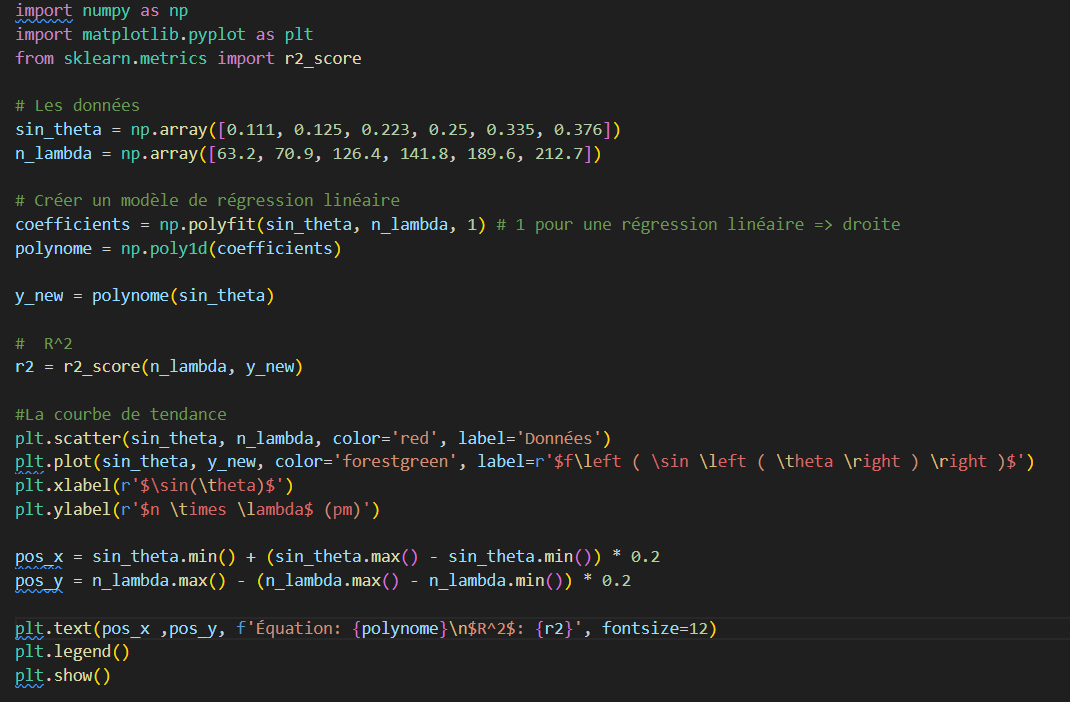
\includegraphics[width=1\linewidth]{Python/Photo_code}
	\caption{Programme Python de la courbe de tendance de $n \times \lambda$ en fonction de $\sin(\theta)$}
	\label{fig:photocode}
\end{figure}


\end{document}